
%% bare_conf.tex
%% V1.4b
%% 2015/08/26
%% by Michael Shell
%% See:
%% http://www.michaelshell.org/
%% for current contact information.
%%
%% This is a skeleton file demonstrating the use of IEEEtran.cls
%% (requires IEEEtran.cls version 1.8b or later) with an IEEE
%% conference paper.
%%
%% Support sites:
%% http://www.michaelshell.org/tex/ieeetran/
%% http://www.ctan.org/pkg/ieeetran
%% and
%% http://www.ieee.org/

%%*************************************************************************
%% Legal Notice:
%% This code is offered as-is without any warranty either expressed or
%% implied; without even the implied warranty of MERCHANTABILITY or
%% FITNESS FOR A PARTICULAR PURPOSE! 
%% User assumes all risk.
%% In no event shall the IEEE or any contributor to this code be liable for
%% any damages or losses, including, but not limited to, incidental,
%% consequential, or any other damages, resulting from the use or misuse
%% of any information contained here.
%%
%% All comments are the opinions of their respective authors and are not
%% necessarily endorsed by the IEEE.
%%
%% This work is distributed under the LaTeX Project Public License (LPPL)
%% ( http://www.latex-project.org/ ) version 1.3, and may be freely used,
%% distributed and modified. A copy of the LPPL, version 1.3, is included
%% in the base LaTeX documentation of all distributions of LaTeX released
%% 2003/12/01 or later.
%% Retain all contribution notices and credits.
%% ** Modified files should be clearly indicated as such, including  **
%% ** renaming them and changing author support contact information. **
%%*************************************************************************


% *** Authors should verify (and, if needed, correct) their LaTeX system  ***
% *** with the testflow diagnostic prior to trusting their LaTeX platform ***
% *** with production work. The IEEE's font choices and paper sizes can   ***
% *** trigger bugs that do not appear when using other class files.       ***                          ***
% The testflow support page is at:
% http://www.michaelshell.org/tex/testflow/



\documentclass[conference]{IEEEtran}
% Some Computer Society conferences also require the compsoc mode option,
% but others use the standard conference format.
%
% If IEEEtran.cls has not been installed into the LaTeX system files,
% manually specify the path to it like:
% \documentclass[conference]{../sty/IEEEtran}


% *** CITATION PACKAGES ***
%
\usepackage{cite}
% cite.sty was written by Donald Arseneau
% V1.6 and later of IEEEtran pre-defines the format of the cite.sty package
% \cite{} output to follow that of the IEEE. Loading the cite package will
% result in citation numbers being automatically sorted and properly
% "compressed/ranged". e.g., [1], [9], [2], [7], [5], [6] without using
% cite.sty will become [1], [2], [5]--[7], [9] using cite.sty. cite.sty's
% \cite will automatically add leading space, if needed. Use cite.sty's
% noadjust option (cite.sty V3.8 and later) if you want to turn this off
% such as if a citation ever needs to be enclosed in parenthesis.
% cite.sty is already installed on most LaTeX systems. Be sure and use
% version 5.0 (2009-03-20) and later if using hyperref.sty.
% The latest version can be obtained at:
% http://www.ctan.org/pkg/cite
% The documentation is contained in the cite.sty file itself.



% *** GRAPHICS RELATED PACKAGES ***
%

\usepackage{graphicx}
\graphicspath{{fig/}}


% *** MATH PACKAGES ***
%
\usepackage{amsmath}
\usepackage{bm}
\usepackage{amssymb}
\interdisplaylinepenalty=2500


% *** ALIGNMENT PACKAGES ***
%
\usepackage{array}

% *** SUBFIGURE PACKAGES ***
\ifCLASSOPTIONcompsoc
 \usepackage[caption=false,font=normalsize,labelfont=sf,textfont=sf]{subfig}
\else
  \usepackage[caption=false,font=footnotesize]{subfig}
\fi

\hyphenation{optical networks semi-conductor}
\usepackage{tikz}
\usetikzlibrary{arrows}

\tikzset{
    left/.style={circle, draw=blue, fill=blue},
    dele/.style={circle, draw=black, fill=black},
    decision/.style={circle, draw=red, fill=red}
}
\begin{document}
%
% paper title
% Titles are generally capitalized except for words such as a, an, and, as,
% at, but, by, for, in, nor, of, on, or, the, to and up, which are usually
% not capitalized unless they are the first or last word of the title.
% Linebreaks \\ can be used within to get better formatting as desired.
% Do not put math or special symbols in the title.
\title{Joint Equalization and Decoding Scheme\\ using Modified Spinal Codes\\ for Underwater Communications}


% author names and affiliations
% use a multiple column layout for up to three different
% affiliations
\author{\IEEEauthorblockN{Yupeng TAI}
\IEEEauthorblockA{State Key Laboratory\\ Acoustics
Institute of Acoustics,\\
Chinese Academy of Sciences \\
Beijing, China}
\and
\IEEEauthorblockN{Frederic GUILLOUD, Christophe LAOT\\ and Raphael LE BIDAN}
\IEEEauthorblockA{SC department\\ 
Telecom Bretagne Institut Mines-Telecom\\ 
Brest, France}
\and
\IEEEauthorblockN{Haibin WANG}
\IEEEauthorblockA{State Key Laboratory\\ Acoustics
Institute of Acoustics,\\
Chinese Academy of Sciences \\
Beijing, China}}

% conference papers do not typically use \thanks and this command
% is locked out in conference mode. If really needed, such as for
% the acknowledgment of grants, issue a \IEEEoverridecommandlockouts
% after \documentclass

% for over three affiliations, or if they all won't fit within the width
% of the page, use this alternative format:
% 
%\author{\IEEEauthorblockN{Michael Shell\IEEEauthorrefmark{1},
%Homer Simpson\IEEEauthorrefmark{2},
%James Kirk\IEEEauthorrefmark{3}, 
%Montgomery Scott\IEEEauthorrefmark{3} and
%Eldon Tyrell\IEEEauthorrefmark{4}}
%\IEEEauthorblockA{\IEEEauthorrefmark{1}School of Electrical and Computer Engineering\\
%Georgia Institute of Technology,
%Atlanta, Georgia 30332--0250\\ Email: see http://www.michaelshell.org/contact.html}
%\IEEEauthorblockA{\IEEEauthorrefmark{2}Twentieth Century Fox, Springfield, USA\\
%Email: homer@thesimpsons.com}
%\IEEEauthorblockA{\IEEEauthorrefmark{3}Starfleet Academy, San Francisco, California 96678-2391\\
%Telephone: (800) 555--1212, Fax: (888) 555--1212}
%\IEEEauthorblockA{\IEEEauthorrefmark{4}Tyrell Inc., 123 Replicant Street, Los Angeles, California 90210--4321}}




% use for special paper notices
%\IEEEspecialpapernotice{(Invited Paper)}




% make the title area
\maketitle

% As a general rule, do not put math, special symbols or citations
% in the abstract
\begin{abstract}
Intersymbol interference (ISI) cancellation over frequency-selective underwater acoustic channel (UAC) is usually performed efficiently using iterative equalization. To this aim, an interleaver is required between the error correction scheme and the modulation scheme, and the longer the interleaver block length the better the performance. However, in the case of time-varying UAC, the length of the interleaver should not be higher than the channel coherence time, thus limiting the performance. Hence, for time-varying UAC with a low coherence time, small interleaver block length have to be used. In this paper, we propose a small block length coding scheme and its associate joint equalization and decoding algorithm based on Spinal codes. We show its efficiency over static large delay spread channels and static UAC: more precisely, simulation results show that the proposed scheme achieves a higher bit error rate than the Turbo equalization scheme with the same block length, especially for high spectral efficiency modulations. Simulations of proposed scheme over UAC obtained from underwater sea experiments are also presented which show the  promising performances.
\end{abstract}

% no keywords




% For peer review papers, you can put extra information on the cover
% page as needed:
% \ifCLASSOPTIONpeerreview
% \begin{center} \bfseries EDICS Category: 3-BBND \end{center}
% \fi
%
% For peerreview papers, this IEEEtran command inserts a page break and
% creates the second title. It will be ignored for other modes.
\IEEEpeerreviewmaketitle


%------------------------------------------------------------------------------------------
\section{Introduction}
% no \IEEEPARstart
Underwater Acoustic Channels (UACs) are known as to be very difficult telecommunication channel, due to time-varying long intersymbol interferences (ISI), making ISI cancellation an active topic for UAC digital communications. Turbo equalization\cite{douillard1995iterative} can be performed to improve the error rate performance for ISI-transmissions: an interleaver is implemented between the error correction scheme and the modulation.
In a turbo-equalization receiver, the performance benefits from the interleaver gain through an iterative process between the equalizer and the decoder. The equalizer produces the estimates of the transmitted symbols using different methods. The maximum likelihood (ML) estimation is the optimal method in getting the minimum bit error rate (BER). However, the complexity of such methods is often to high to be implemented, especially for channels with large delay spread like UACs. Lower complexity equalizer like linear optimization algorithms are then implemented, such as zero forcing (ZF) or minimum mean squared error (MMSE) estimation.
Results shows that the linear MMSE (LE-MMSE) turbo equalizer could completely remove the ISI for a time-invariant frequency-selective channel with an acceptable complexity \cite{laot2001turbo,1006557}, providing that the interleaver block length is sufficiently long as the delay spread of the considered UAC is high. On the other hand, for time-varying channels, increasing the interleaver block length above the coherence time  of the channel will occur a dramatic loss in performance since the channel is usually assumed to be constant for the block length for non-adaptive equalization which is considered in this paper. So the question is: how to improve the equalization performance when the coherence time of the UAC is low, if the interleaver length cannot be increased?

In this paper, a novel joint non-adaptive equalization and decoding scheme based on a modified fixed-rate spinal code is proposed. It aims to provide an acceptable performance for a large range of channels using short block-length codes.  
Spinal codes have been proposed recently in \cite{perry2012spinal} as a new class of non-linear error correction codes based on
random number generators and  pseudo-random hash functions.
There are two aspects within spinal codes which are quite different from popular channel codes. First, an invertible hash function is used which makes graphical or algebraic decoding impossible: the decoding method of spinal code is based on a tree structure algorithm. As the powerful mixing effect of hash function, the near-ML decoder is quite efficient. This is also the foundation of the proposed approximate joint equalization and decoding method achieve an interesting performance-complexity trade-off even for long delay spread channels.  
The second aspect is that the decoding complexity is not increasing when the constellation size of the modulation is increasing. These two features of spinal codes make them a good candidate for joint decoding and equalizing in a single pass, that is to say without the need of iterating the decoding process.

The remainder of this paper is organized as follows: in Section~\ref{sec:TXscheme}, the transmission scheme and the notations are introduced, together with the encoding of Spinal codes. In Section~\ref{sec:jointEqualization}, the joint decoder and equalizer is presented, and the performance results are detailed in Section~\ref{sec:results}. Some conclusions and perspectives are drawn in Section~\ref{sec:conclusion}. 
%------------------------------------------------------------------------------------------
\section{The Transmission Scheme} \label{sec:TXscheme}
\begin{figure}[ht]
\centering
\includegraphics[width=0.9\columnwidth]{tranScheme.pdf}
\caption{The transmission scheme}
\label{fig_tranScheme}
\end{figure}
\begin{figure}[ht]
\centering
\includegraphics[width=1.75 in]{encoderCore.pdf}
\caption{The core hash structure}
\label{fig_hash}
\end{figure}
The transmission scheme is illustrated in Fig.\ref{fig_tranScheme}. Though spinal codes were  proposed as rateless codes, we restrict the spinal code encoder to a fixed code rate denoted $R$. Length-$k$ blocks of independent information bits ${\bm m}$ are fed to a hash function denoted H which produces $k$ length-$v$ binary vector $\bm s_i,\,1\leq i \leq k$, referred to as the seeds. The generation of the seeds can be implemented as an iterative process illustrated in Fig.\ref{fig_hash}. The $k$ bits $m_i$ are fed to the H function which is seeded by $\bm s_{i-1}$. The output is seed $\bm s_i$. The process is initiated by seed $\bm s_0$ which is common to all messages $\bm m$ to be encoded and which is known by the receiver. The set of seeds $\bm s_i$ is then punctured by a factor $p$, meaning that one seed every $p$ seeds is forwarded to the next transmitter function. Hence the transmitted seeds are $\bm s_{pi+1}$ for $1\leq i \leq k$. After puncturing, the remaining seeds are used to feed a random number generator (RNG) to generate $q$ symbols per seed, denoted ${\bm x_i} = \{x_{i,j\}_{1\leq j \leq q}}$ for seed $\bm s_i$. We assume that the cardinal of the constellation is denoted by $2^c$, i.e. each symbol $x_{i,j}$ represents $c$ bits. One possible solution to generate the symbols to be transmitted is illustrated in Fig.\ref{fig_mapper} where the lowest significant bits of the random numbers are mapped to an I/Q constellation mapper.

The coding rate of the transmission is given by $R=kp/cqk=p/cq$, and can thus be tuned over a wide range by varying the puncturing rate $p$, the constellation size $2^c$ or the number of symbols per seed $q$. Fig.\ref{fig_puncturing} illustrates the case where $k=6$, $p=3$ and $q=3$, that is a code rate $R=1/c$.


The symbols $x_{i,j}$ are transmitted over a frequency-selective channel and corrupted by additive white Gaussian noise (AWGN) samples $w_n$ with variance $\sigma^2_w$. Let ${\bm x}$ be the concatenation of all the symbol vectors $\bm x_i$, and let $\bm y$ be vector of all the corresponding received samples. The received signal reads:
\begin{equation}
y_n=\sum_{l=0}^{L-1} h_l x_{n-l}+w_n 
\label{equ_yn}
\end{equation}
where $h_l$ are the coefficients of the discrete channel impulse response of length $L$, $x_n$ and $y_n$ are the $n-$th element of vector $\bm x$ and $\bm y$ respectively, corresponding to the transmission of message $\bm m$.

At the receiver side, the signal-to-noise ration is defined as:
\begin{equation}
\mbox{SNR}=\frac{E_s}{N_0}
\label{equ_snr}
\end{equation}
where $E_s$ is the average energy of $y_n-w_n$ and where $N_0$ is the mono-lateral power spectral density of the Gaussian noise.
% to be continue
% You must have at least 2 lines in the paragraph with the drop letter
% (should never be an issue)	

%------------------------------------------------------------------------------------------
%\section{The Modified Spinal Code} \label{sec:spinalCodes}
%We implement a new kind of fixed-rate spinal code which is less complexity and more suitable for the combination with equalization.
%------------------------------------------------------------------------------------------
%\subsection{Spinal codes Encoding}
%------------------------------------------------------------------------------------------
%\subsubsection{Pseudo-Random Hash Function}
%The core of the spinal code is a recursive structure constructed by a pseudo-random hash function, . As shown in Fig. \ref{fig_hash}, the $H$ takes two inputs: a $v$-bits seed $s_{i-1}$ and one bit of message $m_i$ and returns a $v$-bits seed $s_i$ which is also the next input seed. Additionally, the initial seed value, $s_0$ is a constant value which is known to both the sender and the receiver.

%------------------------------------------------------------------------------------------
%\subsubsection{The Random Mapper}
%
%The set of $k$ seeds ($k$ is the length of the message) is used to seed a random mapper. There is a range of candidate  mapper method for the random mapper: it could be a combination of  a random number generator(RNG) and a usual mapper (constellation mapper for QAM or subcarrier mapper for OFDM, etc.) or directly use the random mapper methods such as Chaotic-FM modulation.
%
%Our implementation is consisted with a random number generator and a constellation mapper as shown in Fig. \ref{fig_mapper} where C-mapper represent the constellation mapper and the $x_{i,1},x_{i,2},...,x_{i,q}$ is the output sub-block of $q$-symbols  under the seed of  $s_i$. Given that the bit per symbol number of mapper output is $c$, then the code rate $R=k/cqk=1/cq$.

%------------------------------------------------------------------------------------------
%\subsubsection{Puncturing}
%As the $q$ is a integer bigger than 1. So the maximum code rate of previous encoding structure is $1/c$ which is quite low when the SNR is high. 
%
%Puncturing maybe a good choice to conquer this problem. Instead of passing all the seeds on the mapper, the sender skips could some of the seeds with a preset puncturing pattern. Given the puncture rate is $p$, the code rate after puncturing turns into $R=p/cq$.
%Benefit from the strongly sequential structure of the encode method. The spinal code could support high puncturing rate. This provide a larger rate adjusting range for the spinal code.
%
%In our implement the puncturing method is a kind of strided puncturing with the consistent strided distance $p$ whose puncturing pattern is $P=[b_1,b_2,...,b_p]$ where only $b_1=1$ and the rests are set to 0. 
\begin{figure}[ht]
\centering
\includegraphics[width=0.9\columnwidth]{mapper.pdf}
\caption{The random mapper}
\label{fig_mapper}
\end{figure}
\begin{figure}[ht]
\centering
\includegraphics[width=3 in]{punturing.pdf}
\caption{The puncturing structure}
\label{fig_puncturing}
\end{figure}
%------------------------------------------------------------------------------------------



%------------------------------------------------------------------------------------------
\section{Joint Decoding and Equalization Scheme} \label{sec:jointEqualization}
%--------------------------------------------------------------------------------------------

\subsection{Near-ML Spinal Code Decoder} \label{sec:nearML}
The best error rate can be obtained by maximum likelihood (ML) decoding when the transmitted information is uniformly distributed.
ML decoding for sequences corrupted by AWGN is obtained by minimizing the euclidean distance between the received sequence and all the possibly transmitted sequences, that is:
\begin{equation}
\widehat{\bm m}=\underset{{\bm m}\in\{0,1\}^k}{\arg\min}\Vert{\bm y}-{\bm x}({\bm m})\Vert^2
\label{equ_ml}
\end{equation}
However the number of operations of ML decoding scales exponentially in $\mathcal{O}(2^k)$ with the information block length. Thus sub-optimal decoding algorithms are of interest. A sub-optimal algorithm for spinal codes decoding is also proposed in \cite{perry2012spinal} which is inspired by a popular complexity reduction named \emph{M-algorithm} \cite{Anderson1984}. The idea is to represent the spinal code encoding process as a bit-wise tree structure. For each new binary information to be encoded, two branches are defined (corresponding to a 0 or 1 information bit) connecting the same tree parent-leaf to 2 child leaves. For each child-leaf, a partial Euclidean distance can be computed. For each new information bit, the number of leaves is multiplied by a factor 2, resulting in $2^k$ leaves in the final tree.

Since the minimum Euclidean distance is to be found, a complexity reduction can be offered by selecting at each new information bit the leaves corresponding to the $B$ lowest Euclidean distances. Fig.\ref{fig_decoderTree} illustrates the complexity reduction algorithm when $B=2$ and $k=4$: the blue leaves represent the leaves corresponding to the lowest partial Euclidean distances, the black ones represent the pruned leaves (when the partial Euclidean distance is too high). The result of the decoder is then the sequence of bits corresponding to the minimum Euclidean distance among the $B$ remaining leaves of the last information bit, and it is illustrated by the red leaves in Fig.\ref{fig_decoderTree}.


%new added
 
%As the  symbols produced by the random-mappers seeded by the same $s_i$ would be coincident with each other, \textbf{y} could be decomposed into $\textbf{y}_1,\textbf{y}_2,...,\textbf{y}_{k/p}$ sub-victors who shares the same seeds. Disregarding the puncturing, the cost function would be:
%\begin{equation}
%\Vert\textbf{y}-\textbf{x}(\textbf{m})\Vert^2=\sum_{i=1}^{k}\Vert\textbf{y}_{i}-\textbf{x}_{i}(s_{i})\Vert^2
%\label{equ_cost0}
%\end{equation}
%Given the addition of $p$-rate strided puncturing and $t =(i-1)p+1$ which is index of the seed who generated $x_i$, the cost function changed into:
%\begin{equation}
%\sum_{i=1}^{\frac{k}{p}}\Vert\textbf{y}_{i}-\textbf{x}_{i}(s_{t})\Vert^2
%\label{equ_cost1}
%\end{equation}
%Further break the sub-vectors $\textbf{y}_i$ into $y_{(i-1)q+1},y_{(i-1)q+2},...,y_{qi}$, we could get the final  cost function:%add explaination
%\begin{equation}
%\sum_{i=1}^{\frac{k}{p}}\sum_{j=q(i-1)+1}^{qi}\vert y_{j}-x_{j}(s_{t})\vert^2
%\label{equ_cost2}
%\end{equation}
%Based on the cost function (\ref{equ_cost2}) and the sequential structure of the encoder.

%The ML decode of spinal code could be recast as a searching for the minimum distant path over a binary tree. The tree is rooted from $s_0$, each node has two edge $e_{m_i}(s_i,s_{i+1})$ connect to two children represent the two possible choices of input bit $m_i$. The total depth of the tree is $k$. So $2^k$ path should be take into count to construct such a binary tree for the optimal ML decoder. This is too complex. 
%
%Fortunately, benefit from the hash function and random generators used, the simply classical approximate ML algorithm which is termed \textit{M-algorithm} in \cite{Anderson1984} shows near optimal performance within linear complexity. The main idea of this algorithm is only maintain $B$ subtrees and prune the rest within each depth increase on the tree. 
%
%Fig. \ref{fig_decoderTree} shows an example of decoder tree with $B$ equal to 2 where the blue node represent the remained, the black nodes represent the pruned and the path consist by red nodes is the final decision of the decoder.%new added

The \emph{M-algorithm} is simple but very efficient in decoding Spinal codes. This is mainly due to the non-linearity and the use of random generator and hash functions which make it possible to increase the distance between two coded sequences corresponding to two messages where most of the bits are identical.
% pairwise independence property of the hash function and the random generators: any pair of messages having the same first information bits and only different from the bits with index higher than $i$ will generated sets of symbols who have the same $iq$ symbols(ignore the puncturing). While their remained subsets are entirely independent with each other.
\begin{figure}
\centering
\begin{tikzpicture}
  [
    grow                    = right,
    sibling distance        = 3cm,
    level distance          = 2cm,
    every node/.style       = {font=\footnotesize},
  ]
  \node [decision] {}
    child { [sibling distance=1.2cm] node [decision] {}
    	child { [sibling distance=1.2cm] node [dele] {}}
    	child { [sibling distance=1.2cm]node [decision] {}
    	    child{node[dele] {}}
    		child{node[decision] {}
    		    child{node[decision]{}}
    			child{node[left]{}}}}}
    child {[sibling distance=1.2cm] node [left] {}
        child {[sibling distance=1.2cm] node [left] {}
            child{node[dele] {}}
    		child{node[left] {}
    			child{node[left]{}}
    			child{node[left]{}}}}
    	child { [sibling distance=1.2cm]node [dele] {}}}
    ;
\end{tikzpicture}
\caption{Tree structure of decoder}
\label{fig_decoderTree}
\end{figure}

\subsection{The Near-ML joint Decoding and Equalization}
The tree-based low complexity decoding algorithm described in Section~\ref{sec:nearML} can be easily adapted to include the equalization step thanks to the knowledge of the channel coefficients which are assumed to be estimated perfectly. Based on Eq.(\ref{equ_ml}) and without considering any seed puncturing ($p=1$), the Euclidean distance is computed by:
%\begin{equation}
%\sum_{i=1}^{\frac{k}{p}}\sum_{j=q(i-1)+1}^{qi}\vert y_{j}-\sum_{l=1}^L x_{j-l}(s_{t})\vert^2
%\label{equ_costEqu}
%\end{equation}
\begin{equation}
\sum_{i=1}^{\frac{qk}{p}}\left\vert y_{i}-\sum_{l=1}^L h_l x_{i-l}\right\vert^2
\label{equ_costEqu}
\end{equation}
%where $t=\lfloor\frac{j-l}{q}\rfloor p+1$.




%--------------------------------------------------------------------------------------------
%\subsection{Time Complexity}
This joint decoding algorithm requires $k$ steps of expanding the tree. Each step expands $2B$ leaves including one hash computations and one Euclidean distance computation. $k/p$ steps involve $q$ random number generations, $Lq$ multiplications to estimate the channel convolution and. The selection for the best $B$ candidates of each step requires $\mathcal{O}(2B)$ operations. The number of required operations per symbol is given in table~\ref{tab_ComplexitySpinal}. 

\begin{table}[!t]
\renewcommand{\arraystretch}{1.3}
\centering
\caption{Number of required operations per symbol of proposed scheme}
\label{tab_ComplexitySpinal}
\begin{tabular}{|c||c|}
\hline
\textbf{operation} &\textbf{amount} \\
\hline
hash\&RNG  & $2B(p+q)/q$\\
\hline
multiplications& $2BL$\\
\hline
comparison & $\mathcal{O}(2Bp/q)$\\
\hline

\end{tabular}

\end{table}

Interestingly, if $B$ is kept constant, the complexity is linear in the message block length $k$ and independent of the number of bit per symbol $c$. Hence, high-order modulations can be implemented without increasing the number of Euclidean distance to compute. 

In comparison,  Turbo equalization requires several iterations between the BCJR \cite{1055186} decoder and LE-MMSE equalization or MAP equalization. The BCJR algorithm for convolution decoder requires $\mathcal{O}(2^{\overline{M}}k)$ operations where $\overline{M}$ is the memory length of the code. LE-MMSE equalization requires $\mathcal{O}((N^2+L^2)k)$ operations, where $N$ is the filter length. The MAP equalization required $\mathcal{O}(2^{cL}k)$ operations. 
%\begin{table}[!hbp]
%\label{tab_ComplexityCompare}
%\centering
%\caption{comparison in number of required operation} 
%\begin{tabular}{|c|c|}
%\hline
%approach & operations\\
%\hline
%proposed scheme & $O(2Bk)$\\
%
%turbo equalization(MAP)& $O((2^{\overline{M}}+2^{cL})k)$\\
%
%turbo equalization(LE-MMSE)& $O((2^{\overline{M}}+N^2+L^2)k)$\\
%\hline
%
%\end{tabular}
%
%\end{table}
With a proper selection of parameters, the proposed scheme requires a  number of operations per symbols comparable to the LS-MMSE Turbo equalization and much more efficient than the MAP Turbo equalization especially when the channel delay is large. 
% The proposed scheme has some additional advantages in efficiency, such it's parallelizable and it could run during the symbol receiving.
%--------------------------------------------------------------------------------------------
\section{Simulation Results} \label{sec:results}
%--------------------------------------------------------------------------------------------
\subsection{Universal Frequency-selective Channel}
%For easily comparing the results with other schemes, the constellation mapper used in random mapper is $M$-QAM mapper.
The universal frequency-selective channels used in this section are proposed in \cite{proakis}:
\begin{equation}
\begin{split}
H_{\mbox{\scriptsize Proakis A}}=&[0.04, -0.05, 0.07, -0.21, -0.5,\\ &0.72, 0.36, 0, 0.21, 0.03, 0.07]^T\\
H_{\mbox{\scriptsize Proakis B}}=&[0.417, 0.815, 0.407]^T\\
H_{\mbox{\scriptsize Proakis C}}=&[0.227, 0.460, 0.688, 0.460, 0.227]^T\\
\end{split}
\end{equation}
\begin{figure}[ht]
\centering
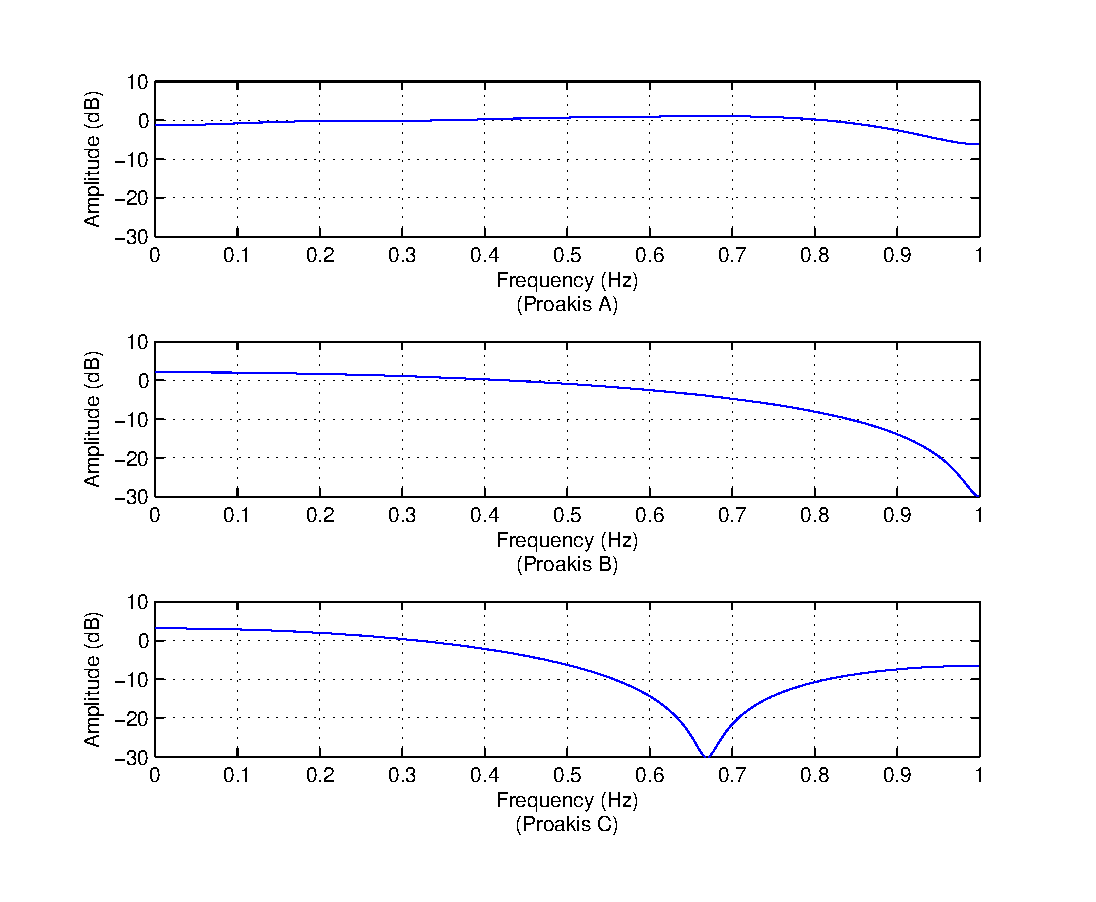
\includegraphics[width=\columnwidth]{PorakisBCchannelResponse.eps}
\caption{The amplitude-frequency responses of the Proakis channel A,B and C}
\label{fig_channel}
\end{figure}
whose amplitude-frequency response is showed in Fig. \ref{fig_channel}.

The parameters for the proposed joint decoding and equalization using spinal codes  are  $k=96, B=1024, q=2, p=2$, yielding a code rate $R=1/2$.
% We found that the modified rate$-1/2$ spinal code with parameters: $k=96, B=1024, q=2, p=2$
Comparison with turbo-equalization are provided to assess to performance-complexity trade-off of our proposed scheme. To this aim, a rate$-1/2$ $163,135$ (expressed in octals) convolution code whose memory length is 6 has been implemented. QPSK signaling is used for both schemes.
% over AWGN channels. So they are selected respectively to apply into the proposed scheme and Turbo equalization for comparing there performance over frequency-selective channel.  
\begin{figure}[ht]
\centering
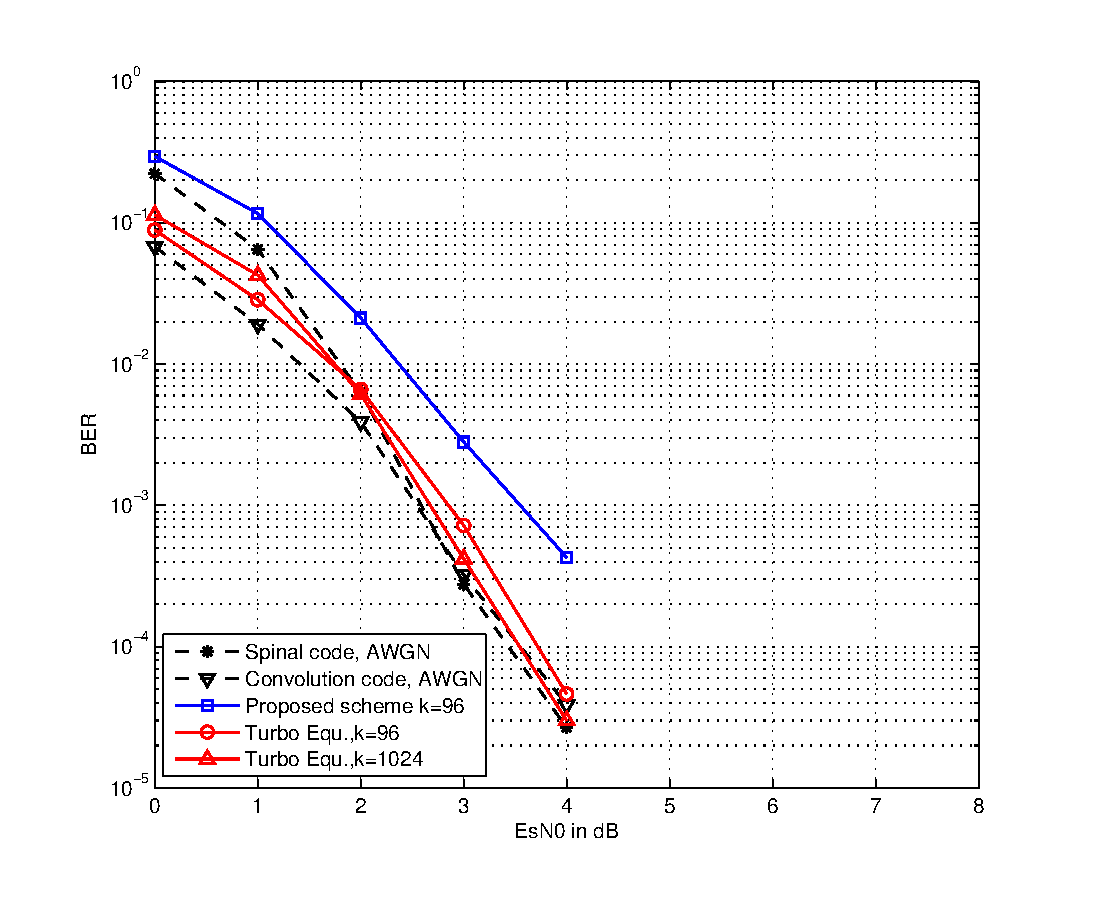
\includegraphics[width=\columnwidth]{ChAQPSKComparison.eps}
\caption{The performance of proposed scheme and Turbo equalization over Proakis A channel for QPSK modulation}
\label{fig_ChAQPSKComparison}
\end{figure}
\begin{figure}[ht]
\centering
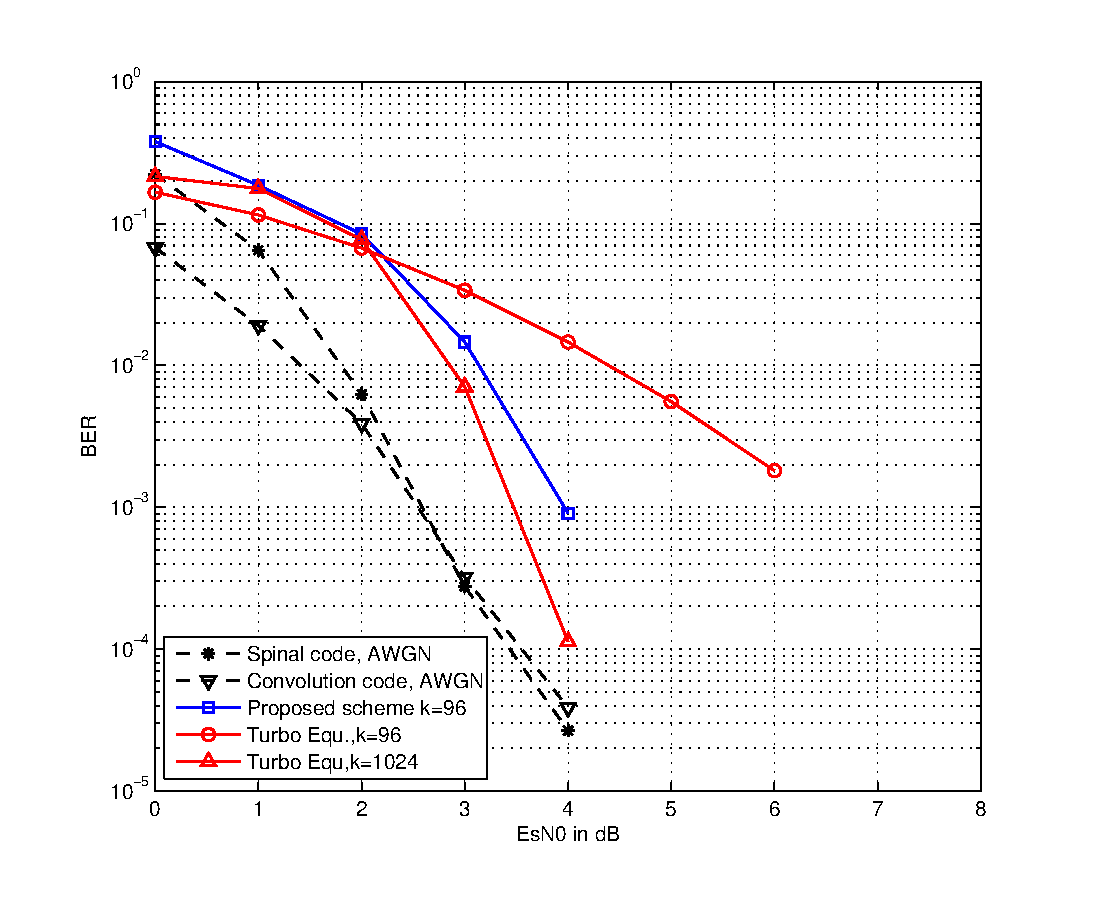
\includegraphics[width=\columnwidth]{ChBQPSKComparison.eps}
\caption{The performance of proposed scheme and Turbo equalization over Proakis B channel for QPSK modulation}
\label{fig_ChBQPSKComparison}
\end{figure}
\begin{figure}[ht]
\centering
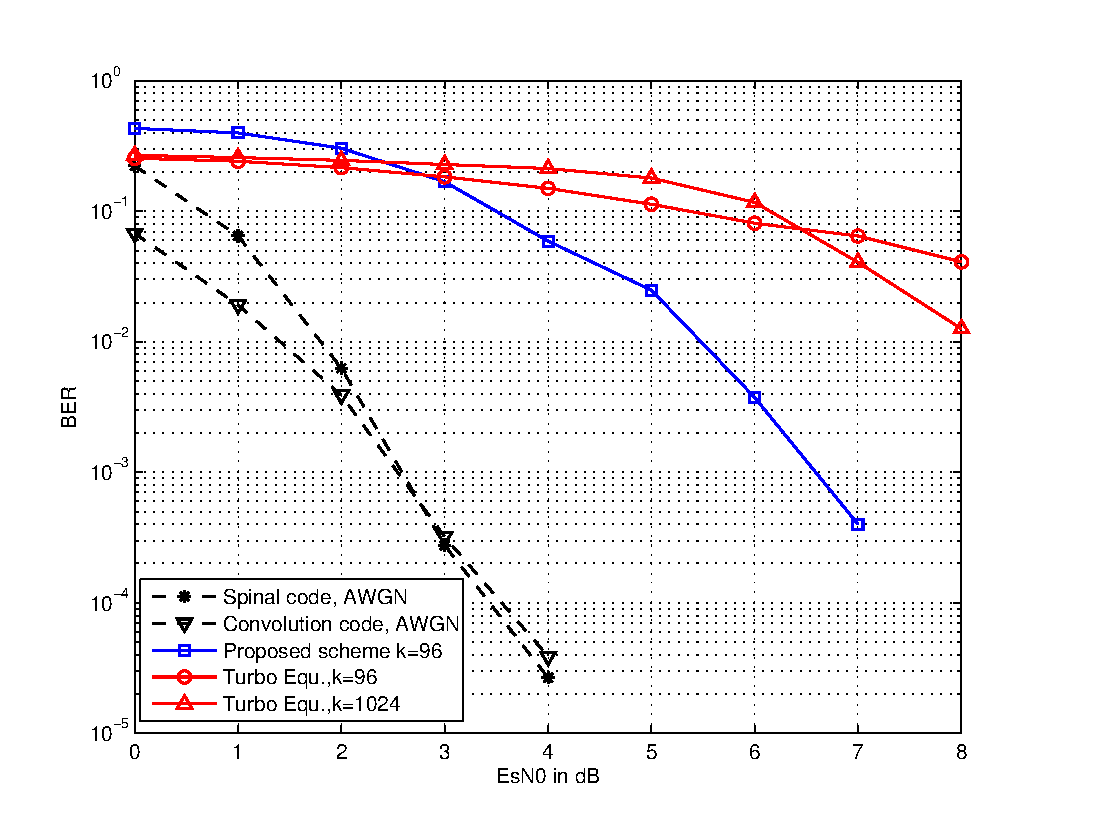
\includegraphics[width=\columnwidth]{ChCQPSKComparison.eps}
\caption{The performance of proposed scheme and Turbo equalization over Proakis C channel for QPSK modulation}
\label{fig_ChCQPSKComparison}
\end{figure}

Fig. \ref{fig_ChAQPSKComparison}, Fig. \ref{fig_ChBQPSKComparison} and Fig. \ref{fig_ChCQPSKComparison}  present the performance of the proposed scheme and comparison with Turbo equalization after 5 iterations over Proakis A,B and C channel respectively. The results show that the proposed scheme outperforms turbo-equalization when the block length is short for highly frequency-selective channels.
However, a performance loss to the theoretical bound is observed with the lower frequency-selective channel, due to the sub-optimal equalization.
% requires more time complexity to erase the final gap to the theoretical bound.
\begin{figure}[!t]
\centering
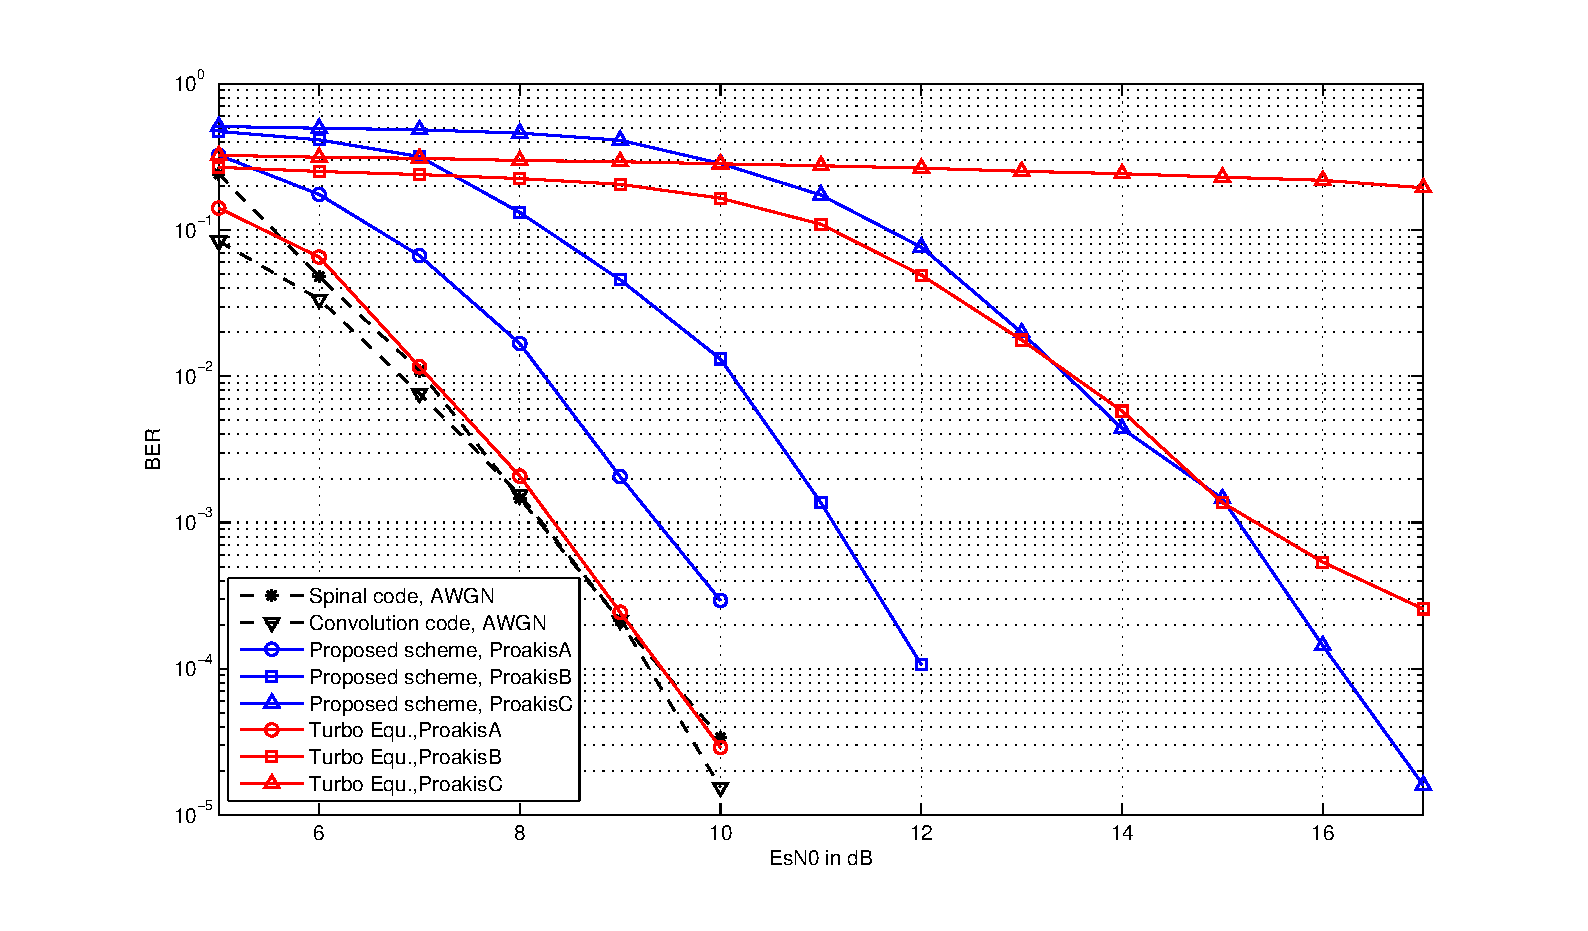
\includegraphics[width=\columnwidth]{16QAMComparison.eps}
\caption{The performance of proposed scheme and Turbo equalization at the fifth iteration for $16-$QAM modulation}
\label{fig_16QAMComparison}
\end{figure}

Fig. \ref{fig_16QAMComparison} shows the performances of the proposed scheme for $16-$QAM signaling and its comparison with Turbo equalization.
As $c$ is increased, the puncturing factor is set to $p=1$ to keep the code rate $R=1/2$. We can see that the performance gap between our proposed scheme and Turbo equalization over Proakis B and Proakis C channel increases compared to QPSK signaling. For these highly frequency-selective channels, it becomes more difficult for the turbo equalization to get a reliable feedback of the estimated data for low SNR, which is not the case for the porposed scheme.
%Whereas the proposed scheme isn't a iterate structure, so their is no "BER threshold" problem.%This is just my analise. Don't know if it's reasonable.

%--------------------------------------------------------------------------------------------
\subsection{Underwater Acoustic Channels Extracted from Sea Experiment}

%-------------------------------------------------------------------
\subsubsection{Shallow Sea Underwater Acoustic Channel}
This channel is estimated from the data of an underwater acoustic communication experiment carried out on the South China Sea in 2011 by the Institute of Acoustic (IOA), Chinese Academy of Sciences (CAS). The channel coefficients and  amplitude-frequency responses are represent in Fig. \ref{fig_ShallowChannel}. The channel amplitude-frequency response is smooth except for a notch at the normalized frequency 0.2. 
\begin{figure}[ht]
\centering
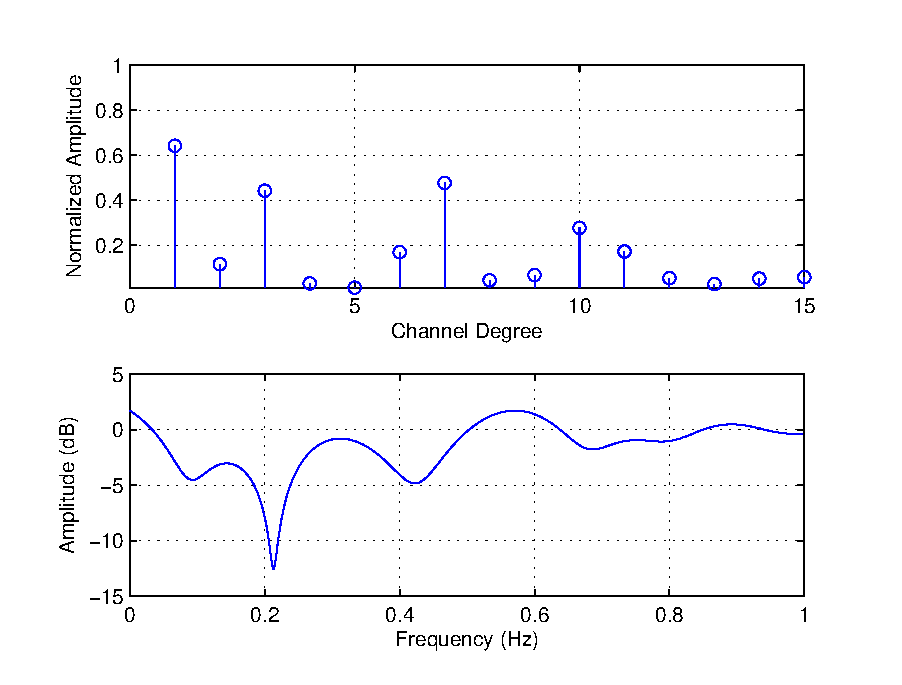
\includegraphics[width=\columnwidth]{ShallowChannel.eps}
\caption{The amplitude-time and amplitude-frequency responses of a shallow-sea UAC}
\label{fig_ShallowChannel}
\end{figure}
The performance of the proposed scheme and the Turbo equalization over this channel is compared in Fig.\ref{fig_ShallowQPSKComparison}. The proposed scheme also shows stable performance with small block length.
\begin{figure}[ht]
\centering
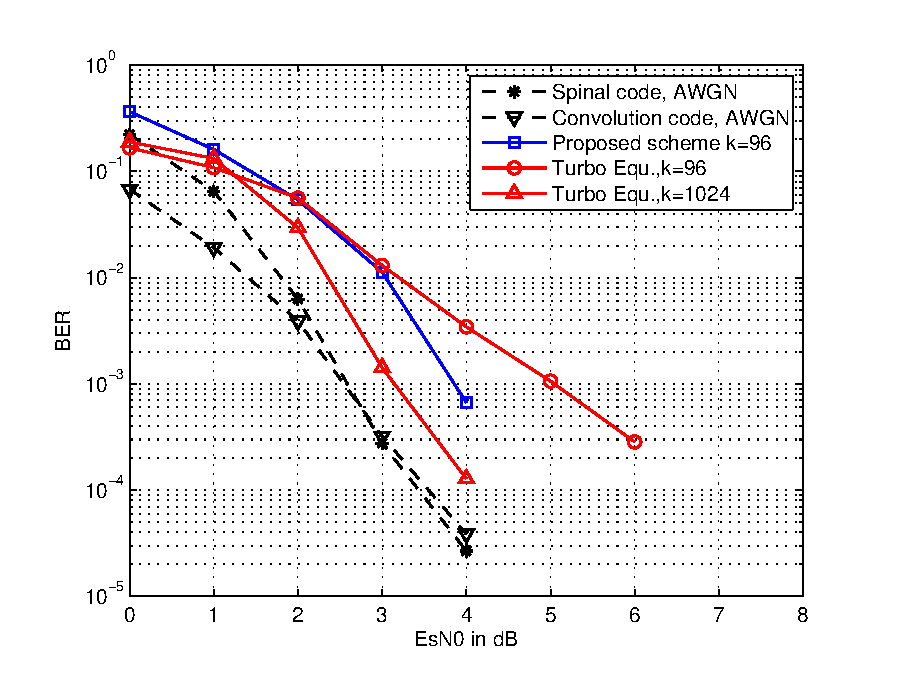
\includegraphics[width=\columnwidth]{ShallowQPSKComparison.eps}
\caption{The performance of the proposed scheme and Turbo equalization over shallow-sea UAC}
\label{fig_ShallowQPSKComparison}
\end{figure}
%--------------------------------------------------------------------------
\subsubsection{Deep Sea Underwater Acoustic Channel}
Fig.\ref{fig_DeepChannel} shows the deep sea channel extracted from the data of an experiment carried out in South China Sea in 2013 by IOA, CAS. The water depth of the experiment area is 5000m. The distance between the transmitter and the receiver is 69km which is exactly in the second  shadow area of the transmission loss curve. The channel is affected by a severe multipath with a delay of 100 symbol periods.

\begin{figure}[ht]
\centering
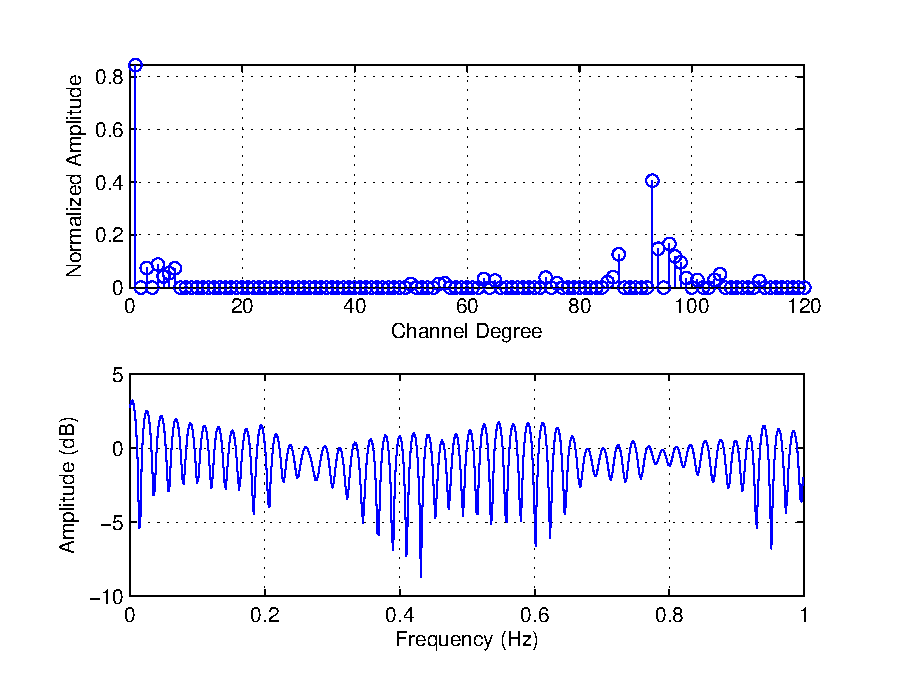
\includegraphics[width=\columnwidth]{DeepChannel.eps}
\caption{The amplitude-time and amplitude-time responses of deep-sea underwater acoustic channel}
\label{fig_DeepChannel}
\end{figure}
The performance comparison is illustrated in Fig.\ref{fig_DeepQPSKComparison}.

\begin{figure}[ht]
\centering
\includegraphics[width=\columnwidth]{DeepQPSKComparison.eps}
\caption{The performance of proposed the scheme and Turbo equalization over deep-sea UAC}
\label{fig_DeepQPSKComparison}
\end{figure}

%One thing to be mentioned, the filter length of Turbo Equalization is  set to 120 to equal with the channel length.  I'm not sure if it is the proper method to deal with the large delay channel? Would a equalization with such long filter practicable? So I don't know if we should drop this simultaion. I just want to show that complexity for such a large delay channel is still acceptable. But I found it's hard to assess it. 

\section{Conclusion} \label{sec:conclusion}
This paper presents the design and performance analysis of a modified spinal code used for underwater acoustic transmissions, together with a joint equalization and decoding scheme. A tree-based suboptimal decoding algorithm is implemented with lower complexity, where decoding and equalization are performed jointly on a non-time varying underwater acoustic channel (UAC). This non-iterative receiver scheme shows stable and acceptable performance for a larger range of channels when small block lengths are considered. The performance gap between the proposed scheme and the LE-MMSE turbo equalization is as large as 6dB over the highly frequency-selective Proakis B channel using 16QAM modulation method. 

The aim of implementing small length transmission blocks is then to provide efficient transmission schemes on fast time-varying UAC. The perspective of this work relies mainly in implementing the proposed transmission scheme for time-varying UAC and also to apply adaptive equalization for further comparisons.

%This paper shows a newly attempt to overcome the ISI in UAC with a limited code block length. It also leaves aspect to explore for the future work. First, the approximate is not perfect enough to remove all ISI totally. The performance always leaves a small gap to the theoretical bound. Second, the addition of channel estimation and the performance analysis for time-varying channels is also interesting to explore. The last but not the least, the coding scheme is newly designed, their is a bunch of similar structure and realizations. It's also interesting to seek the one for better overcoming the channel ISI of UAC.






\bibliographystyle{IEEEtran}
\bibliography{IEEEabrv,OceanConf_full}

\end{document}


